%% Copyright (c) 2004  SciSoft.  All rights reserved.
%%
%% This file is part of CGAL (www.cgal.org); you may redistribute it under
%% the terms of the Q Public License version 1.0.
%% See the file LICENSE.QPL distributed with CGAL.
%%
%% Licensees holding a valid commercial license may use this file in
%% accordance with the commercial license agreement provided with the software.
%%
%% This file is provided AS IS with NO WARRANTY OF ANY KIND, INCLUDING THE
%% WARRANTY OF DESIGN, MERCHANTABILITY AND FITNESS FOR A PARTICULAR PURPOSE.
%%
%% 
%%
%% Author(s)     : Fernando Cacciola <fernando_cacciola@hotmail.com>

\begin{ccRefConcept}{EdgeCollapsableMesh}

\ccSetThreeColumns{xxx}{xxxxxxxx}{}
%% \ccHtmlCrossLink{}     %% add further rules for cross referencing links
%% \ccHtmlIndexC[concept]{} %% add further index entries

\ccDefinition

The concept \ccRefName\ describes the requirements for the type of 
triangulated surface mesh that can be passed to the
simplification algorithm.

The surface must be structurally equivalent to a polyhedral surface
having only triangular faces. 
It can have any number of connected components, boundaries 
(borders and holes) and handles (arbitrary genus).

\ccRefines
\ccc{HalfedgeGraph}

\ccHeading{Valid Expressions}

The mesh simplification algorithm requires the free function \ccc{collapse_triangulation_edge}.

  \ccTagFullDeclarations
  %\def\ccLongParamLayout{\ccTrue}
  \ccFunction
  {template<class EdgeCollapsableMesh>
  typename boost::graph_traits<EdgeCollapsableMesh>::vertex_descriptor
  halfedge_collapse(typename boost::graph_traits<EdgeCollapsableMesh>::edge_descriptor const& ue
                   , EdgeCollapsableMesh& mesh);
  }  
  {Collapses the undirected edge \ccc{(v0v1,v1v0)} replacing it with \ccc{v0} or \ccc{v1},
  as described in the following paragraph.
  \ccPrecond This function requires \ccc{mesh} to be an oriented 2-manifold with or without boundaries. Furthermore, the undirected edge \ccc{(v0v1,v1v0)} must satisfy the {\em link 
  condition} \cite{degn-tpec-98}, which guarantees that the surface is also 2-manifold after the edge collapse. }

\smallskip
Let \ccc{v0} be the source and \ccc{v1} be the target vertices of \ccc{v0v1}.

For \ccc{e} $\in \{$ \ccc{v0v1,v1v0} $\}$, let \ccc{en} and \ccc{ep} be the next and previous 
edges, that is \ccc{en = next_edge(e, mesh)}, \ccc{ep = prev_edge(e,mesh)}, and let 
\ccc{eno} and \ccc{epo} be their opposite edges, that is 
\ccc{eno = opposite_edge(en, mesh)} and \ccc{epo = opposite_edge(ep,mesh)}.

Then, after the collapse of \ccc{(v0v1,v1v0)} the following holds:

\begin{itemize}
\item The edge \ccc{e} is no longer in \ccc{mesh}.
\item One of $\{$\ccc{v0,v1}$\}$ is no longer in \ccc{mesh} while the other remains.
\footnote{Even though it would appear that v0 can always be the vertex being removed, there is a case when removing the edge \ccc{e} {\em requires} \ccc{v1} to be removed as well. See figure \ref{CollapseFigure5}.}
Let \ccc{vgone} be the removed vertex and \ccc{vkept} be the remaining vertex.
\item If \ccc{e} was a border edge, that is \ccc{get(is_border, e, mesh) == true}, then \ccc{next_edge(ep) == en}, and \ccc{prev_edge(en) == ep}.
\item If \ccc{e} was not a border edge, that is \ccc{get(is_border, e, mesh) == false}, then \ccc{ep} and \ccc{epo} are no longer in \ccc{mesh} while \ccc{en} and \ccc{eno} are kept in \ccc{mesh}.
\item For all edges \ccc{ie} in \ccc{in_edges(vgone,mesh)}, \ccc{target(ie,mesh) == vkept} and \ccc{source(opposite_edge(ie),mesh) == vkept}.
\item No other incidence information has changed in \ccc{mesh}.
\end{itemize}

The function returns vertex \ccc{vkept} (which can be either \ccc{v0} or \ccc{v1}). 

\begin{figure}[htpb]
\begin{ccTexOnly}
\begin{center}
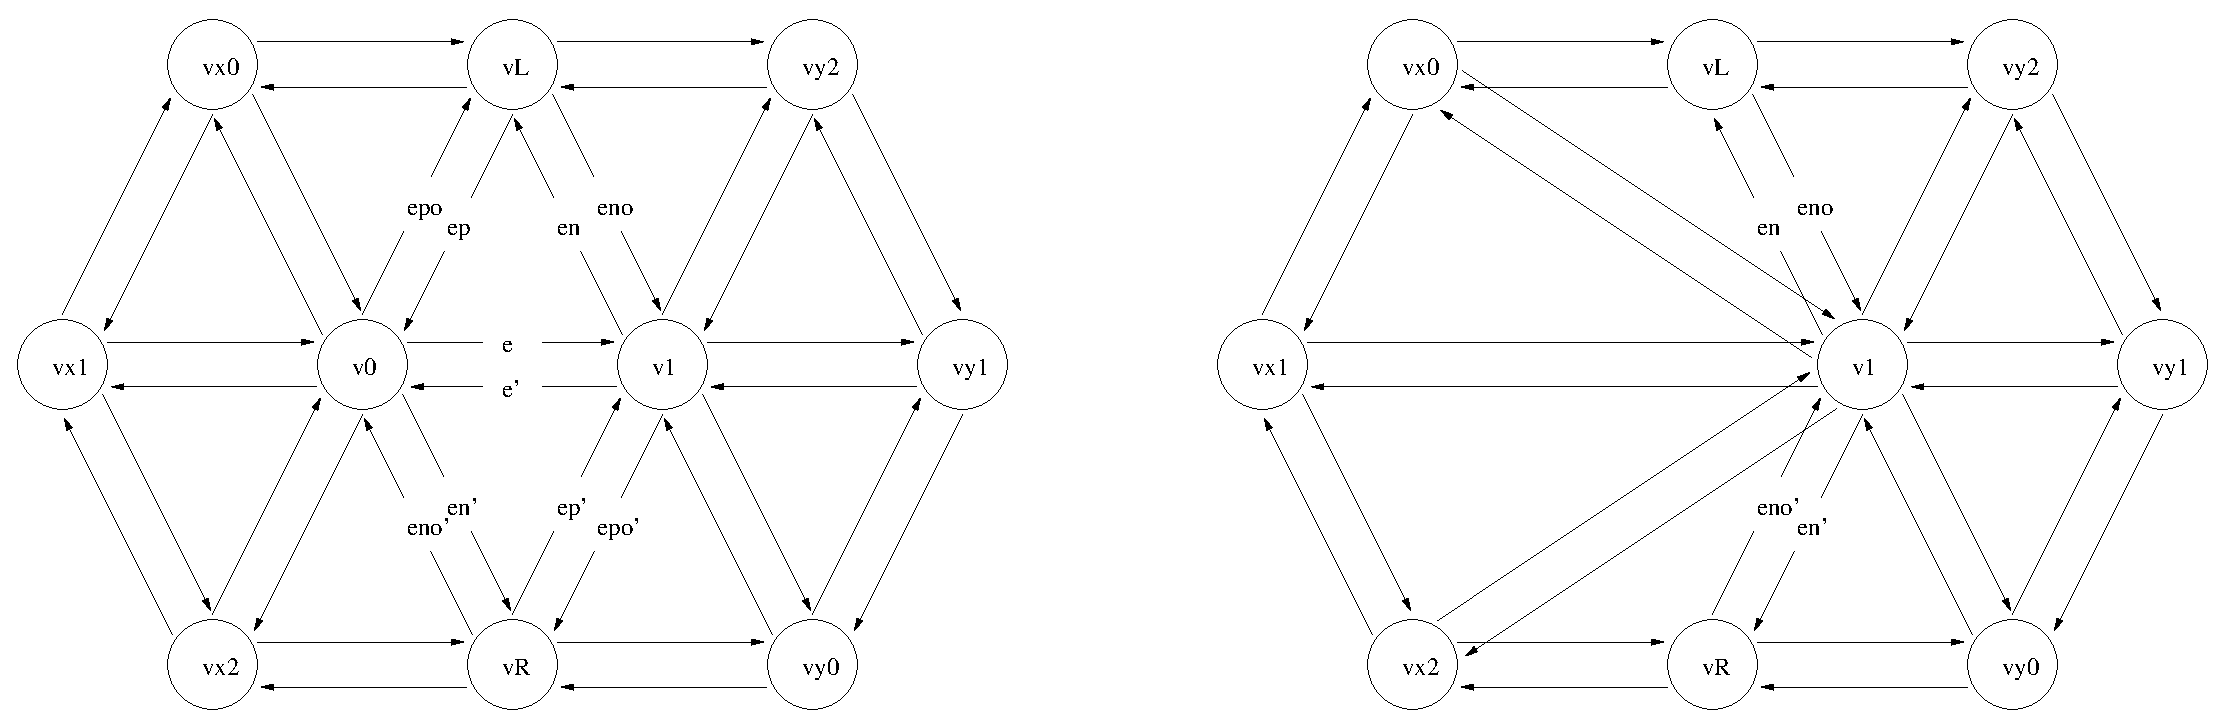
\includegraphics[width=17cm]{Surface_mesh_simplification_ref/fig/general_collapse} % omit suffix .eps to support PS and PDF
\end{center}
\end{ccTexOnly}
\begin{ccHtmlOnly}
<TABLE CELLSPACING=40>
<TR>
<CENTER>
<IMG BORDER=0 SRC="./fig/general_collapse.png" ALIGN=middle ALT="Simplification illustration">
</CENTER>
</TR>
</TABLE>
\end{ccHtmlOnly}
\caption{General case. The following mesh elements are removed: triangles ($v0,v1,vL$) and ($v1,v0,vR$), edges $(e,e')$, $(ep,epo)$ and $(ep',epo')$, and vertex $v0$.}
\end{figure}



\begin{figure}[htbp]
\begin{ccTexOnly}
\begin{center}
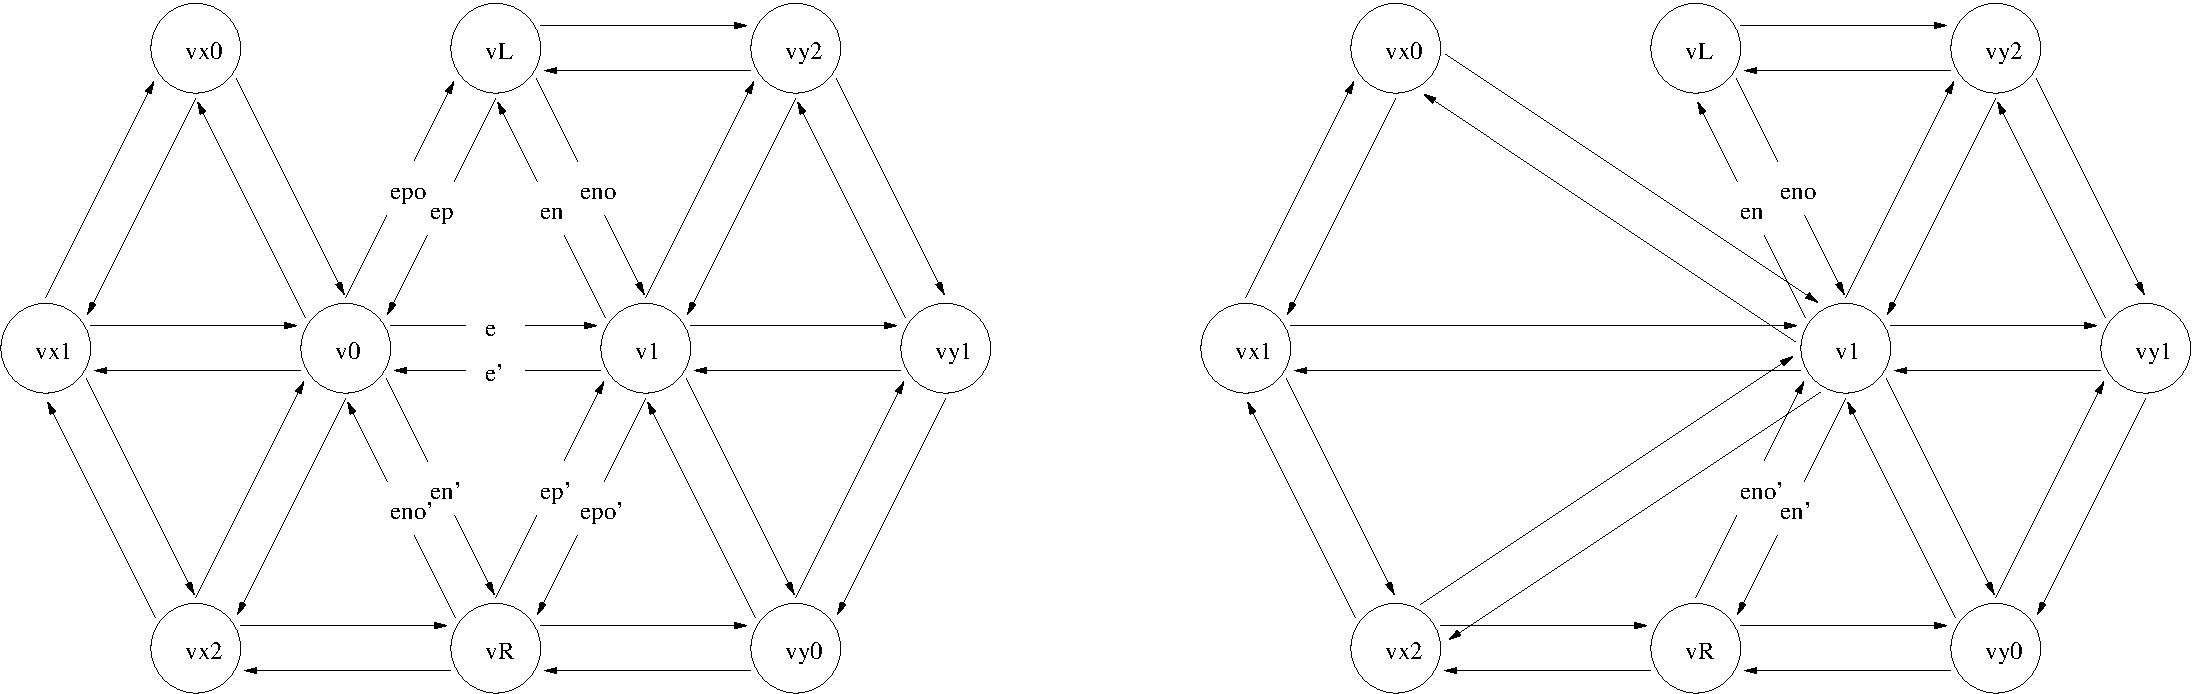
\includegraphics[width=17cm]{Surface_mesh_simplification_ref/fig/border_collapse3} % omit suffix .eps to support PS and PDF
\end{center}
\end{ccTexOnly}
\begin{ccHtmlOnly}
<TABLE CELLSPACING=40>
<TR>
<CENTER>
<IMG BORDER=0 SRC="./fig/border_collapse3.png" ALIGN=middle ALT="Simplification illustration">
</CENTER>
</TR>
</TABLE>
\end{ccHtmlOnly}
\caption{When the collapsing edge is not itself a border, but is incident upon a border edge that is removed, the operation is the same as in the general case.}
\end{figure}

\begin{figure}[htbp]
\begin{ccTexOnly}
\begin{center}
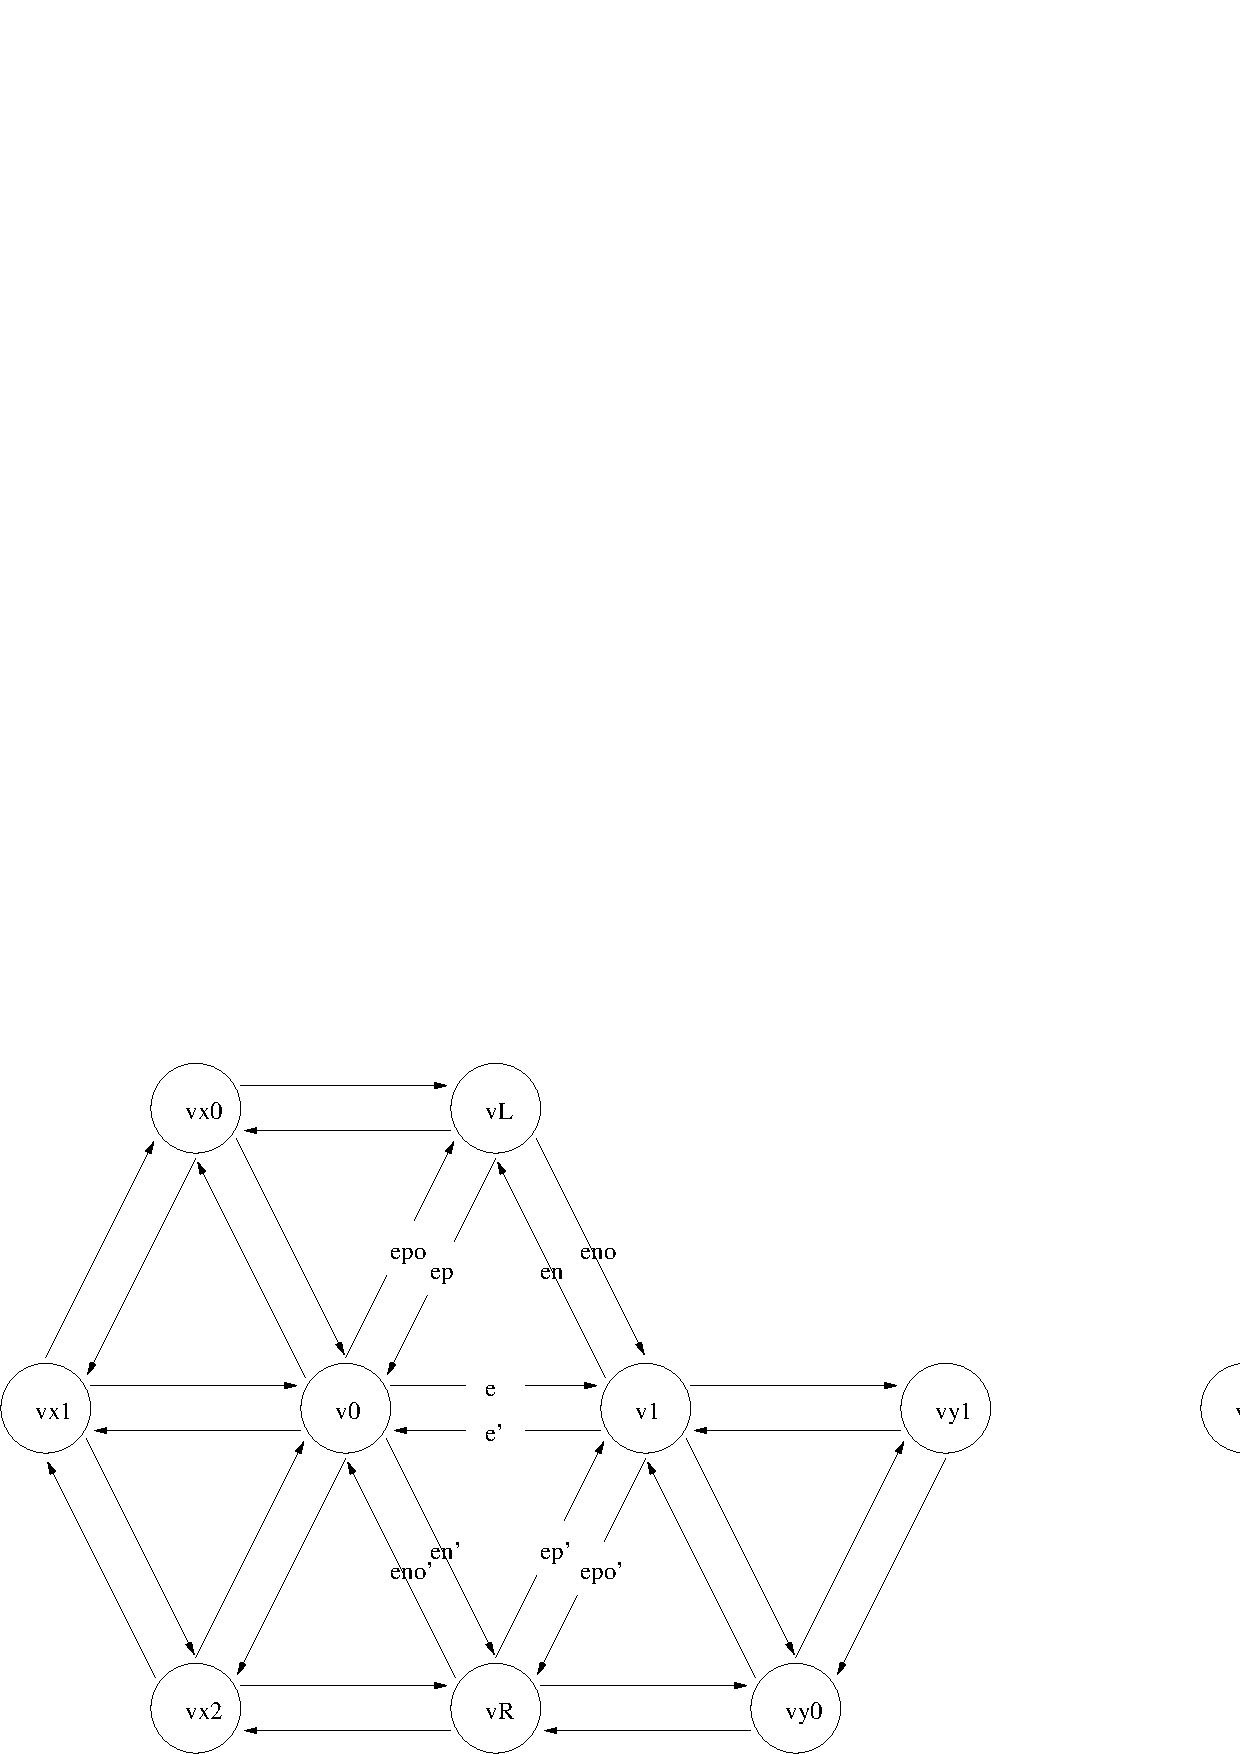
\includegraphics[width=17cm]{Surface_mesh_simplification_ref/fig/border_collapse2} % omit suffix .eps to support PS and PDF
\end{center}
\end{ccTexOnly}
\begin{ccHtmlOnly}
<TABLE CELLSPACING=40>
<TR>
<CENTER>
<IMG BORDER=0 SRC="./fig/border_collapse2.png" ALIGN=middle ALT="Simplification illustration">
</CENTER>
</TR>
</TABLE>
\end{ccHtmlOnly}
\caption{When the collapsing edge is not itself a border, but is incident upon a border edge that is {\em not} removed, the operation is still the same as in the general case.}
\end{figure}

\begin{figure}[htbp]
\begin{ccTexOnly}
\begin{center}
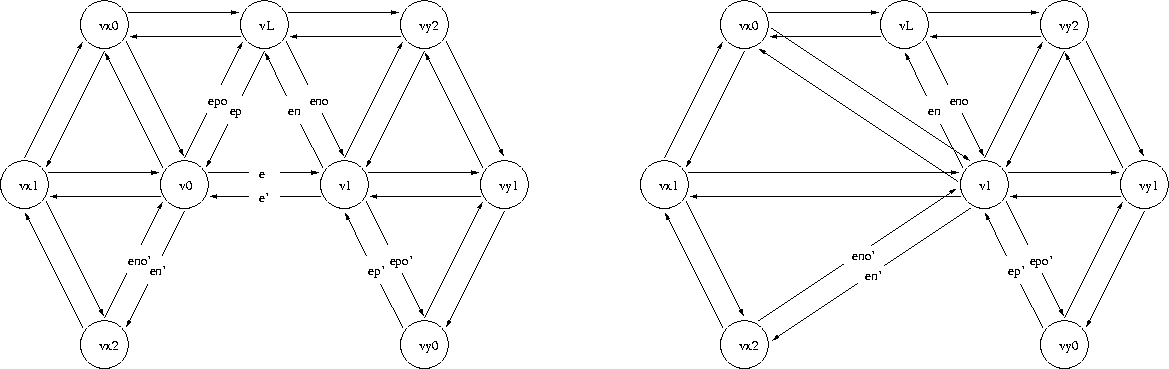
\includegraphics[width=17cm]{Surface_mesh_simplification_ref/fig/border_collapse1} % omit suffix .eps to support PS and PDF
\end{center}
\end{ccTexOnly}
\begin{ccHtmlOnly}
<TABLE CELLSPACING=40>
<TR>
<CENTER>
<IMG BORDER=0 SRC="./fig/border_collapse1.png" ALIGN=middle ALT="Simplification illustration">
</CENTER>
</TR>
</TABLE>
\end{ccHtmlOnly}
\caption{When the collapsing edge is itself a border, only 1 triangle is removed. Thus, even if $(ep',epo')$ exists, it's not removed.}
\end{figure}

\begin{figure}[htbp]
\begin{ccTexOnly}
\begin{center}
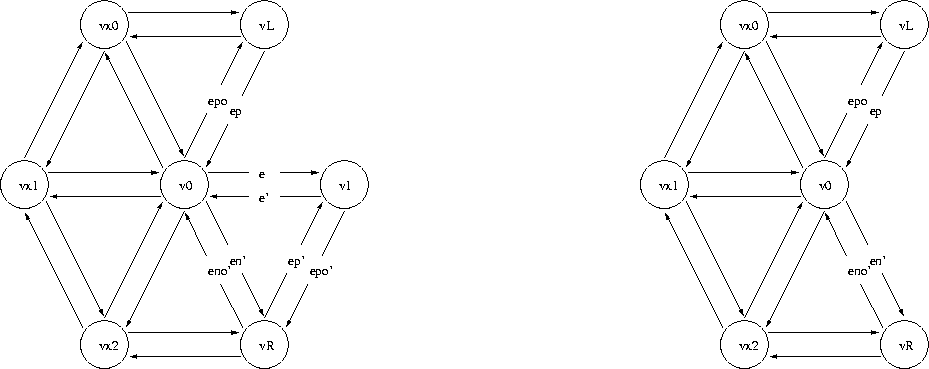
\includegraphics[width=17cm]{Surface_mesh_simplification_ref/fig/border_collapse4} % omit suffix .eps to support PS and PDF
\end{center}
\end{ccTexOnly}
\begin{ccHtmlOnly}
<TABLE CELLSPACING=40>
<TR>
<CENTER>
<IMG BORDER=0 SRC="./fig/border_collapse4.png" ALIGN=middle ALT="Simplification illustration">
</CENTER>
</TR>
</TABLE>
\end{ccHtmlOnly}
\caption{This figure illustrates the single exceptional case when removing $(v0,v1)$ neccesarily implies removing $(v1)$, thus $(v0)$ remains.}
\label{CollapseFigure5}
\end{figure}

\ccHasModels
\ccRefIdfierPage{CGAL::Polyhedron_3<Traits>}\\
(If it has only triangular faces, and via
{\em External Adaptation}, which is described in \cite{cgal:sll-bgl-02}
and this {\sc Bgl} web page: \path|http://www.boost.org/libs/graph/doc/leda_conversion.html|).

\ccSeeAlso
\ccRefIdfierPage{boost::graph_traits< CGAL::Polyhedron_3<Traits> >}\\
\ccRefIdfierPage{CGAL::halfedge_graph_traits< CGAL::Polyhedron_3<Traits> >}

\end{ccRefConcept}

% +------------------------------------------------------------------------+
%%RefPage: end of main body, begin of footer
% EOF
% +------------------------------------------------------------------------+
